\documentclass[12pt]{article}

\usepackage{graphicx}
\usepackage[sorting=none]{biblatex}
\usepackage[margin=1in]{geometry}
\usepackage[colorlinks=true]{hyperref}
\usepackage{amsmath}
\usepackage{amssymb}
\usepackage[format=plain, labelfont=it, font=footnotesize, labelsep=period]{caption}

\addbibresource{references.bib}

\title{Pendulum Lab Report 1}
\author{Kevin (Zerui) Wang}
\date{\today}

\begin{document}

\pagenumbering{gobble}

\maketitle

\pagenumbering{arabic}

\section{Introduction}
The first part of this lab report focuses on the relationship the period and release angle of a simple pendulum. After results were collected and analyzed, an improved version of the pendulum was created to collect angular data in order to determine the Q factor.

\section{Background} \label{Background}
For a simple pendulum with a mass $m$ hanging from a string with length $L$ experiencing a downwards force due to gravity $g$, the period, for a release angle $\theta$, is given by the following equation \cite{the-simple-pendulum}:
\begin{equation} \label{eq:eq1}
    2\pi \sqrt{\frac{L}{g}}
\end{equation}

This is otherwise known as the small angle approximation of a pendulum, which only holds if $\theta \lesssim 20^{\circ}$ \cite{the-simple-pendulum} (This phenomena may be observed if one were to release the pendulum from a large $\theta$). For $\theta \gtrsim 20^{\circ}$, a new model must be created to take into account the realistic behaviour of a pendulum, namely a second order differential equation with respect to $\theta$:
\begin{equation} \label{eq:eq2}
    \frac{d^2\theta}{dt^2} + \frac{g}{L}\sin{\theta} = 0
\end{equation}
Which must be solved numerically where the solution to Equation \ref{eq:eq2} diverges from simple harmonic motion that could accurately predict the motion of a pendulum under small angle approximation \cite{the-simple-pendulum}. It may also be useful to note that the $m$ term does not come up in any of these equations, which implies pendulum period does not depend on mass.

Additionally the existence of air resistance and friction within the string fibres will cause a dampening effect on the oscillation of a pendulum. This effect can be modeled given an initial angle $\theta_0$ in radians, decay constant $\tau$, a pendulum period $T$, and a angular phase shift $\phi$ \cite{damped-oscillations}:
\begin{equation}
    \theta(t) = \theta_0 e^{-{t/\tau}} \cos\left(2\pi\frac{t}{T} + \phi_0\right)
\end{equation}

In order to quantify the dampening effect of a pendulum, its Q factor may be used, defined as follows for a damped oscillator [need citation]:
\begin{equation}
    Q = \pi\frac{\tau}{T}
\end{equation}
Another way of measuring the Q factor is counting the number of oscillation it takes for the amplitude to decay to $e^{-\pi} \approx 4\%$, or measuring $Q/n$ where the amplitude decays to $e^{-{\pi/n}}$ its original.

This way of determining the Q factor works because when $Q = n\pi\frac{\tau}{T}$, $t = \frac{QT}{n}$. The amplitude would them be $e^{-{t/T}} = e^{-{\pi/n}}$

\section{Period and Release Angle}

\subsection{Experimental Setup}
The initial setup for the pendulum was made by first attaching a protractor on a desk. The pendulum, made by threading a piece of cotton string around a stainless steel quick link, was then placed at the center of the protractor. The length of the pendulum was measured using measuring tape. An image of the experimental setup is shown below:

\begin{figure}[!hptb]
    \centering
    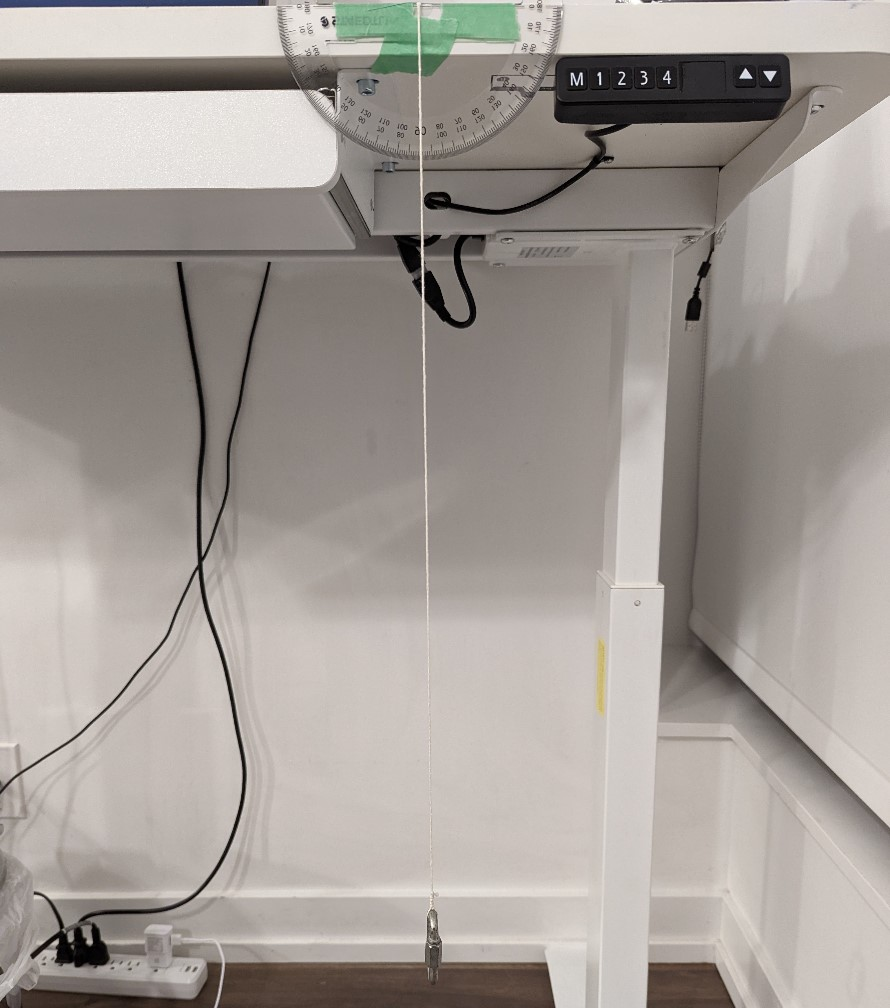
\includegraphics[width=0.5\textwidth]{../figures/exp_setup1.jpg}
    \caption{\centering Picture of experimental setup for period vs. release angle data collection}
    \label{fig:figure 1}
\end{figure}

\newpage

\subsection{Data}
The data collected for the period vs. release angle graph is shown in the plot below:

\begin{figure}[!hptb]
    \centering
    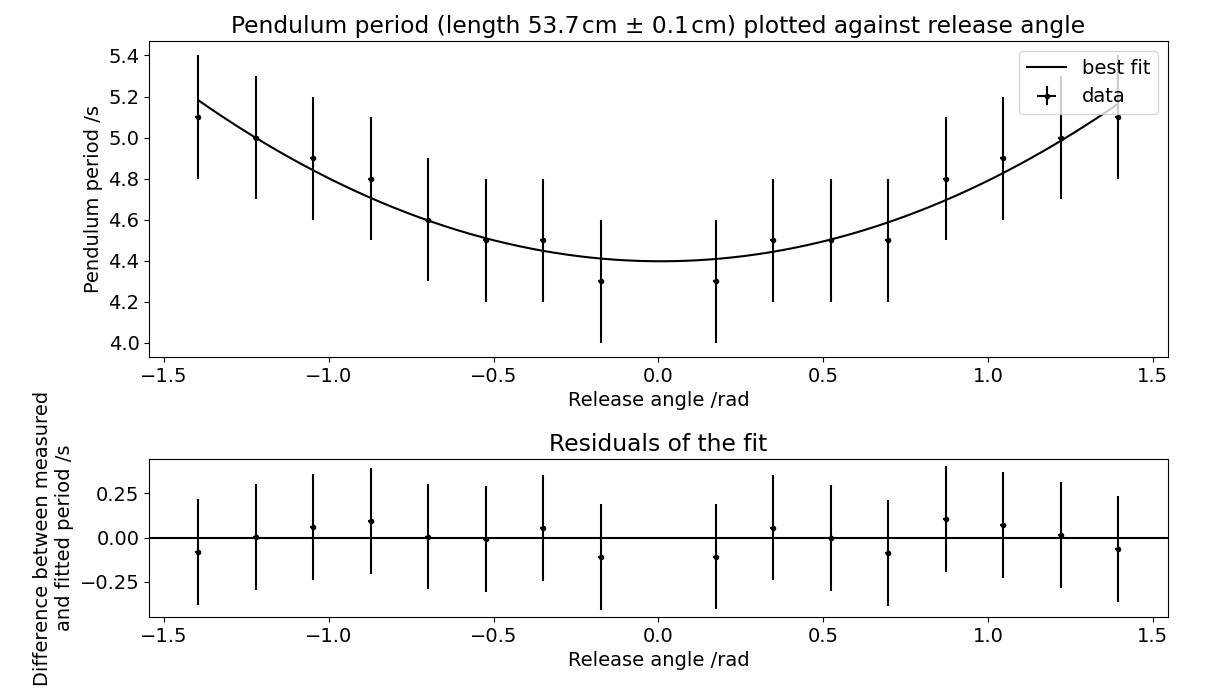
\includegraphics[width=\textwidth]{../figures/period_vs_release_angle.png}
    \caption{\centering Period plotted against release angle}
    \label{fig:figure 2}
\end{figure}

All data collected for this graph were done without the need for tracking software. The uncertainty for the protractor was taken to be the smallest increment, $0.5^{\circ}$ converted to radians, and the period uncertainty was taken to be the average human reaction time, $0.25\,\text{s}$ \cite{reaction-time}.

\subsection{Analysis}
- power series passes thru uncertainties
- mention what range is small enough
- equation 1 would imply that \ref{eq1}
- Provide a clear conclusion about whether your pendulum's period depends on ampli- tude. If you do find some dependence, you should clearly indicate what range (if any) of amplitudes are `small enough' that the value of C can be ignored. Be clear as to what criteria you used to make a `small enough' judgment. \ref*{Background}
- talk about asymmetry

\section{Finding the Q Factor}
- [objective] fix for asymmetry

\subsection{Experimental Setup}
- was improved with the v
\subsection{Data}
- data collected using tracker
\subsection{Comparing Q Factors}
\subsection{Analysis}
- this is gonna be an exponential fit because the overall residuals are smaller than when the fit is linear [include a figure containing both]
- Describe how you took this data (specifically including the impact of the Q factor on your choices)

\section{Notes}


\begin{itemize}
    \item period is dependent on angle \cite*{what-is-yeast}
    \item If you find that the period does depend on the angle, and you find that your Q factor is not huge (in the 1000s), then you will need to be careful about how you measure the period. (i.e. conclusions of Q factor based on angle?)
    \item compare the ``3'' ways of calculating the Q factor
\end{itemize}


\textbf{Procedure}\\
for version 2 of the pendulum, I got rid of a swinging motion by attaching 2 strings

asymmetry can be tested by taking residuals?

talk about uncertainties (make a section for it?)

\begin{equation}
    \theta(t) = 0.86 e^{-{\tau/30}} \cos\left(2 \pi \frac{t}{1.43} - 0.08\right)
\end{equation}

\section*{Conclusion}

\newpage

\printbibliography

\end{document}
